\documentclass[12pt,a4paper]{article}

\usepackage[T1,T2A]{fontenc}
\usepackage[utf8]{inputenc}
\usepackage[english,russian]{babel}
\usepackage{microtype}
\usepackage{csquotes}
\usepackage{amsmath}
\usepackage{amsthm}
\usepackage{amssymb}
\usepackage{mathtext}
\usepackage{physics}
\usepackage{newfloat}
\usepackage{caption}
\usepackage{indentfirst}
\usepackage{titlesec,titletoc}
\usepackage{geometry}
\usepackage{hyperref}
\usepackage{mdframed}
\usepackage[inline]{enumitem}
\usepackage{graphicx}
\usepackage{subfig}
\usepackage[titletoc,toc]{appendix}

\DeclareGraphicsExtensions{.pdf,.png,.jpg,.PNG}
\graphicspath{{./img/}}
\captionsetup[figure]{justification=centering}
\renewcommand{\thesubfigure}{\asbuk{subfigure}}
\DeclareCaptionLabelSeparator{dotseparator}{. }
\captionsetup{labelsep=dotseparator}
\geometry{left=1cm,right=1cm,top=2cm,bottom=2cm}
\makeatletter\appto{\appendices}{\def\Hy@chapapp{Appendix}}\makeatother
\renewcommand{\appendixtocname}{Приложения}
\renewcommand{\appendixpagename}{Приложения}

\DeclareMathOperator{\Rot}{\mathbf{rot}}
\DeclareMathOperator{\Grad}{\mathbf{grad}}
\DeclareMathOperator{\Div}{\mathbf{div}}
\DeclareMathOperator{\D}{D}
\newcommand{\V}[1]{\mathbf{#1}}
\newcommand{\Op}[1]{\hat{\V{#1}}}


\title{Сферические резонаторы}
\author{Василевский А.В.}

\begin{document}

    \maketitle
    \tableofcontents

    \section{Постановка задачи}

    %
    %
    %
    %%%%%%%%%%%%%%%%%%%%%%%%%%%%%%%%%%%%%%%%%%%%%%%%%%%%%%%%%%%%%%%%%%%%%%%
    %                           SUBSECTION                                %
    %%%%%%%%%%%%%%%%%%%%%%%%%%%%%%%%%%%%%%%%%%%%%%%%%%%%%%%%%%%%%%%%%%%%%%%
    %
    %
    %

    \subsection*{Введение}

        В данной части работы будет изложено введение в сферические резонаторы и их термодинамику.

        Изучение термодинамики подобных структур важно для современной микроэлектроники, оптики и других наук, оперирующих со сферически симметричными малоразмерными структурами. В частности, оно позволяет получить более или менее точные количественные оценки мешающих факторов~--- тепловых шумов, а также указать возможные способы компенсации их воздействия.

        Общим предметом рассмотрения работы станут сферические резонаторы, ограниченные идеально проводящими стенками. Будет получен вид векторных сферических мод, описана методика их получения. Исходя из этого будет получена спектральная плотность энергии, запасенной в резонаторе.

    %
    %
    %
    %%%%%%%%%%%%%%%%%%%%%%%%%%%%%%%%%%%%%%%%%%%%%%%%%%%%%%%%%%%%%%%%%%%%%%%
    %                           SUBSECTION                                %
    %%%%%%%%%%%%%%%%%%%%%%%%%%%%%%%%%%%%%%%%%%%%%%%%%%%%%%%%%%%%%%%%%%%%%%%
    %
    %
    %

    \subsection{Сферические микрорезонаторы}

        Неотъемлемым элементом почти любого сложного оптического и микроволнового прибора является резонатор. Именно прогресс в совершенствовании резонаторов зачастую приводил к достижению качественно новых результатов. Так, появление мазеров и лазеров было бы невозможно без реализации высокодобротных резонаторов СВЧ и оптического диапазонов. Высокодобротные резонаторы активно используются для сужения и стабилизации линии генерации, в качестве фильтров и дискриминаторов, в разнообразных высокочувствительных сенсорах и датчиках, в метрологии и в прецизионных физических экспериментах. \cite{microresonators}

        Так, одним из ключевых направлений развития физики сегодня является квантовая теория измерений и связанный с ней интерес к манипуляциям с отдельными квантовыми объектами. Резонаторы играют существенную роль в этих исследованиях. Именно с помощью миниатюрных высокодобротных резонаторов в оптическом диапазоне были впервые продемонстрированы неклассические состояния электромагнитного поля и были впервые проведены впечатляющие эксперименты по наблюдению эффектов взаимодействия отдельных фотонов и отдельных атомов. Тесно связаны с этим направлением и такие, вызывающие активное внимание и ожидания, приложения, как квантовые компьютеры, квантовая криптография и квантовая телепортация. Одним из основных требований для наблюдения квантовых эффектов является изоляция системы от внешнего классического мира и уменьшение в ней диссипации для замедления распада состояний (декогеренции), что означает для резонаторов повышение добротности. \cite{microresonators}

        Взаимодействие излучения со сферическими телами исследуется уже более 100 лет. В последние десятилетия, в связи с обнаружением сверхузких резонансов рассеяния и возможностью создания на этой основе микрорезонаторов с гигантской добротностью, открывающих новые горизонты оптической микрофотоники, интерес к этому вопросу усилился многократно. \cite{microresonators}

        Повышенный интерес к микрорезонаторам и бурное развитие области сверхдобротных резонаторов ставят перед наукой и другие задачи. Всесторонний анализ различных путей диссипации энергии в микрорезонаторах с целью повышения их добротности и стабильности является задачей, требующей особого внимания. Для микроэлектронных приборов, элементов квантовых компьютеров и т.д. не менее важным является вопрос устранения шумов. Тепловые шумы являются довольно серьезным мешающим фактором. Генерация этих шумов на сферических микроструктурах тоже требует изучения в целях их учета и компенсации.

        На \autoref{fig:spherical_resonator} показан сферический микрорезонатор с МШГ (моды шепчущей галереи). В виде пояса видна спекл-картина рассеяния на поверхностных неоднородностях поля МШГ.
        %
        \begin{figure}[h]
            \centering
            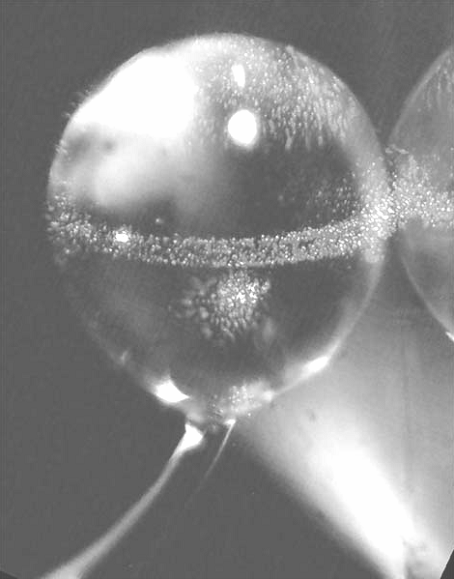
\includegraphics[width=0.5\textwidth]{spherical_resonator}
            \caption[]{Оптический сферический микрорезонатор на ножке рядом с возбуждающей призмой, в которой видно его отражение. Диаметр около $570$ мкм, добротность $> 10^9$. Физический факультет МГУ \cite{microresonators}}
            \label{fig:spherical_resonator}
        \end{figure}

    %
    %
    %
    %%%%%%%%%%%%%%%%%%%%%%%%%%%%%%%%%%%%%%%%%%%%%%%%%%%%%%%%%%%%%%%%%%%%%%%
    %                        BIBLIOGRAPHY                                 %
    %%%%%%%%%%%%%%%%%%%%%%%%%%%%%%%%%%%%%%%%%%%%%%%%%%%%%%%%%%%%%%%%%%%%%%%
    %
    %
    %

    \nocite{*}
    \bibliographystyle{../../lib/doc/bib/utf8gost705s}
    \bibliography{../../lib/doc/bib/resonators}

\end{document}
